% !TEX root = ../main.tex
\section{Introduction}
\label{introduction}

There is overwhelming anecdotal evidence that data scientists spend at least 80\%
of their time finding, preparing, integrating and cleaning data sets.
% that they wish to analyze. 
The remaining 20\% of their time is spend doing the actual desired 
analysis tasks.
% which comprise their job description.  
One data officer (Mark Schrieber of
Merck) estimates the number is 98\%, in which case data scientists spend less
than one hour a week on tasks in their job description.

In this paper we present the architecture of Data Civilizer, a system under
construction at MIT, QCRI and Waterloo, whose purpose is to lower the ``mung work'' 
faced by data scientists.  In the rest of this section we present overall architecture of the \dcv system, and we describe the
environment at Merck to motivate the components of Data Civilizer.  
%We also indicate an architecture diagram of our system.   
Sections~\ref{sec:discovery}--\ref{sec:workflow} present the
components of our system, followed in Section~\ref{sec:wild} by experiences ``in the wild'' at
both Merck and the MIT Data Warehouse.  We expect to present a demo at CIDR
of our system running in the MIT environment.  Finally, Section~\ref{sec:workflow} draws
conclusions and suggests next steps.

\subsection{Architecture}

\dcv is a stack of modules that address three main tasks: {\em Discovery}, 
{\em Linkage} and  {\em Polystore Query Processing}. Figure~\ref{fig:arch} shows the general architecture of the \dcv system. The discovery layer to the underlying slew of available data sets and data bases is what search engines is to the internet; the module is responsible for defining meaningful data units, collecting meta data and other semantic information around each of these units, and provide basic relationship among these units to build a data fabric similar in spirit to a web knowledge graph \cite{DBLP:conf/semweb/AuerBKLCI07,DBLP:conf/sigmod/BollackerEPST08,DBLP:conf/www/SuchanekKW07}. The output graph is later used by the linkage layer to find more complex relationship that allow stitching these units together to answer a wide range of analytic queries against ad-hoc schemas. The linkage layer focuses primarily on exploring the large space of possible ``join graphs'' that connect the underlying data sets. For example, discovering (often fuzzy) Primary key-foreign key relationship between tables, and more generally various forms of inclusion dependency, which allow for joining or stitching these raw data sources together to populate an analytics schema or a view. Since these raw data sets often live in a variety of systems (often know as a ploystore) and have different levels of trustworthiness and soundness (how clean they are), the query answering layer in \dcv uses the space of possible join graphs constructed by the linkage layer, and the available meta data from the discovery layer to populate an specific schema or a view on-demand in the polystore environment.   


The three layers in \dcv have different scale and response time constraints, which greatly affect the design and the choice of algorithms in each layer: The discovery layer is ``always on'' working in the background to find, index and mine connections among large number of data sets, hence, almost-linear algorithms that work on a Big data scale is a key requirement. At the same time, the discovery layer is not expected to have on-line response time and will be mostly performing off-line batch data processing workflows focusing primarily on discovering simple and basic connections and relationships among the various data artefacts. On the other hand, the linkage layer has to find more complex relationships, such as inclusion dependencies, which are too expensive to run on the full scale raw data. Hence, the linkage layer has to judiciously use the graph output of the discovery layer to scope the search space. While the linkage layer has an off-line component that focuses on mining these complex join relationships, efficient use of the query submitted o the query processing layer can help pruning the large space of possible join graphs. Finally, the polystore query processing layer has the tightest response time constraints to respond within reasonable time to ad-hoc analytics against often continuously changing analytics schemas (views). Limiting the space of possible data stitching strategies, while taking into account the polystore execution environment is a key technical challenge. 


\begin{figure}
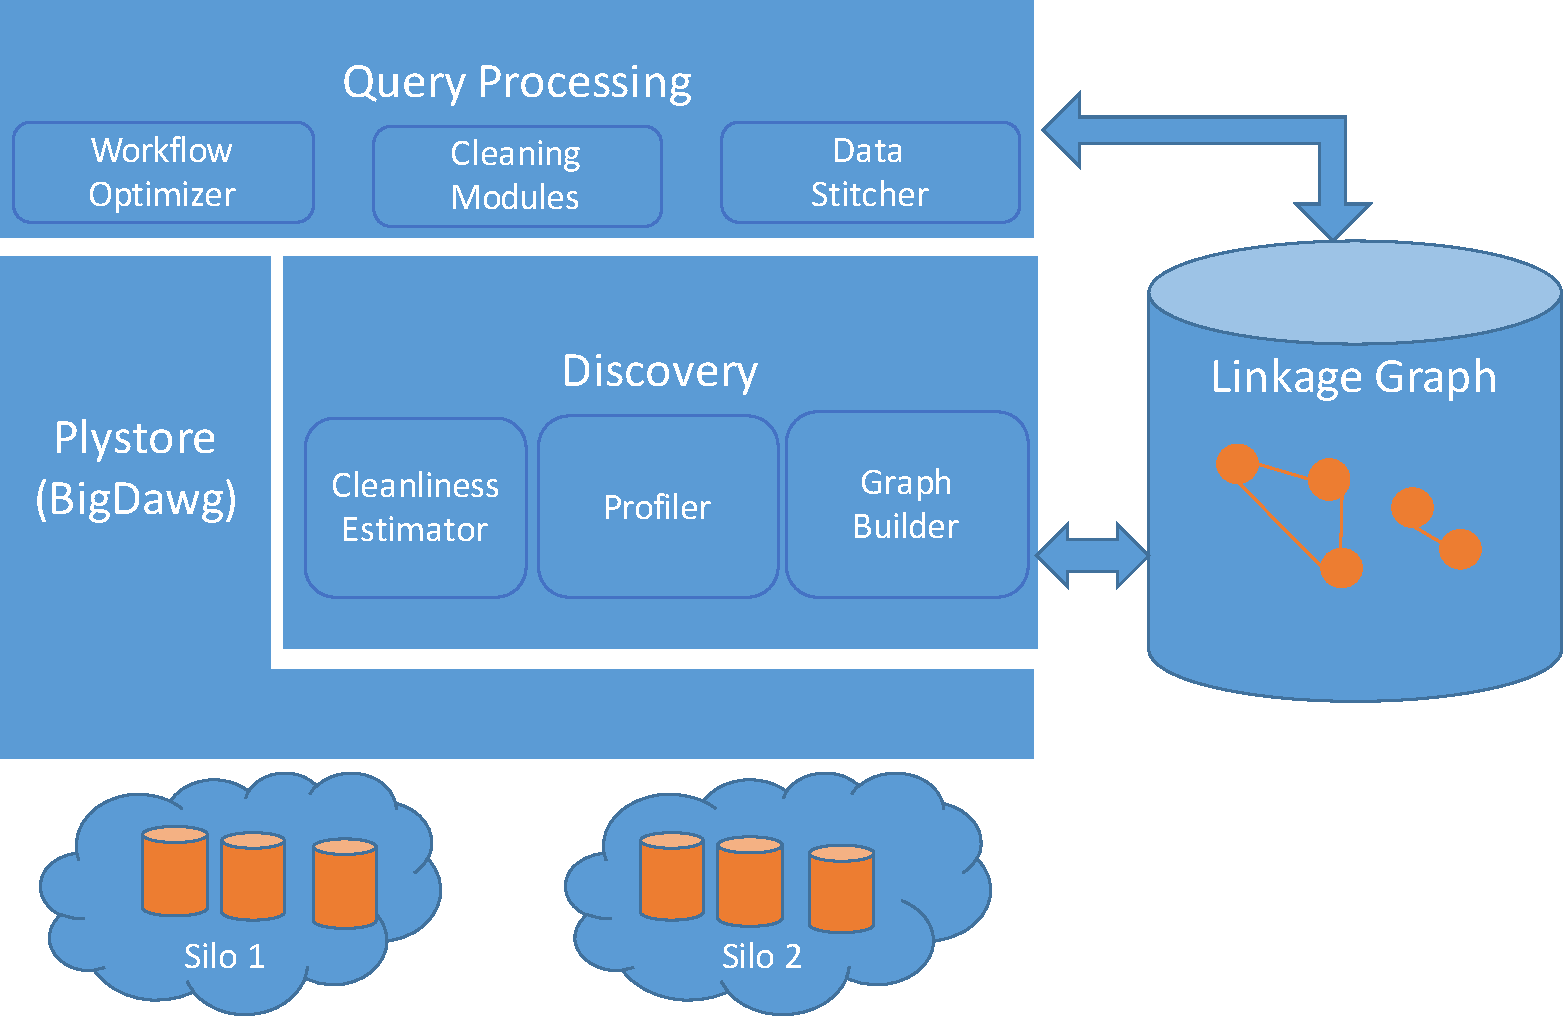
\includegraphics[width=3.5in]{arch2.pdf}
\caption{\dcv Architecture}
\label{fig:arch}
\end{figure}

    

\subsection{Merck Environment}

Merck is a large decentralized drug company with about XXX employees, of which
YYY are data scientists.  An exemplar data scientist would come up with a
hypothesis, for example the drug ritalin causes brain cancer in rats weighing
more than 1Kg.  His first job is to identify data sets, both within the Merck
firewall and outside that might contribute to resolving this question.  Inside
the firewall, Merck has some 4000 Oracle databases and countless other
repositories in which relevant data might reside.  Data Civilizer has a
Discovery component, discussed in Section~\ref{sec:discovery}, 
which assists the scientist with finding data sets of interest.

Data sets identified by the Discovery module are invariably linked together by
intermediary data sets.  Hence, the next step is to construct ``data stitching''
paths among all of the data sets identified during discovery.  This task is the
job of the Data Stitcher, which is discussed in Section~\ref{sec:stitching}. One can think of the
output of the data stitcher as one or more views on the underlying data. It is
now necessary to perform data curation on these multiple views.  This entails
extracting data from source data storage systems, performing schema integration
on the multiple views, transforming data into a common representation, cleaning
erroneous values from the source data sets, and performing entity consolidation
on resulting records.  Our Data Tamer system\cite{DBLP:conf/cidr/StonebrakerBIBCZPX13} dealt with schema integration
and entity consolidation.  More recently, we wrote a system DataXformer~\cite{DBLP:conf/icde/AbedjanMIOPS16}
which supported transformations, and we examined a collection of data cleaning
systems~\cite{evaluatioin}.

Since Merck has a variety of data storage systems and exascale data volumes, it
is simply not reasonable to move all data to a central ``central lake'. Also, it is
not reasonable to perform data curation up front on enterprise data, as was
advocated by Data Tamer.  Instead Data Civilizer must be a pull-based system
that does data curation on demand, as data scientists need to access data to get
their work done.  Therefore, Data Civilizer must be based on a polystore
architecture~\cite{DBLP:journals/sigmod/DugganESBHKMMMZ15}, that can pull data out of multiple underlying storage
engines on demand.  Obviously, data cleaning, data transformation and entity
consolidation must be integrated with querying the polystore.  In this way, a
key technical optimization is to push filters and joins through cleaning
operations and into the underlying data storage system wherever possible.  The
merger of polystores and data curation steps is discussed in Section~\ref{sec:curating}, and we
term the resulting system a Curating Polystore.  

Optimizing such a curating polystore is the subject of the next two sections.
Materializing views is very expensive, because of the human effort involved,
when automatic algorithms are unsure of what to do.  Therefore, we must estimate
the cost of constructing the MV, because a scientist may not have the budget to
pay for the human effort involved.  This is the topic of Section~\ref{sec:cleanliness}.  It entails
constructing a model for how dirty the data in the source data sets actually is.
An ancillary topic is to estimate the cleanliness that can be achieved for a
given budget for cleaning activities.  In this way, a scientist can decide
whether or not he wishes to proceed with the project at hand.

Moreover, it is silly to discard expensive-to-construct materialized views (MV)
after their initial use by a data scientist.  Hence, we assume that they are
generally retained for future use.  Moreover, future MVs may be based off
previously constructed ones or on original data sources.  As a result, there may
be several ways to construct a new MV, with differing costs and available
accuracy (since each existing MV has some given accuracy, as noted above.
Therefore, the data stitching problem must be revisited to deal with this
materializiation cost/accuracy tradeoff.  This is the subject of Sections~\ref{sec:enhancedstitching}.

Section~\ref{sec:updates} then turns to update issues.   If a source data set is updated, then
updates must be incrementally propagated through the data curation pipeline to
update downstream MVs.  In some cases, the human effort involved may be
daunting, and the MV should be discarded rather than updated.  Lastly, if a
scientist updates his MV, we must propagate changes to other descendent data
sets, as well as back upstream to data sources. 

Section~\ref{sec:workflow} then turns to our workflow system, whereby a data scientist can
iterate over our components in whatever order he wishes, undo previous workflow
steps, and perform alternate branching from given MVs. 

We then turn in Section~\ref{sec:wild} to the current implementation status of Data Civilizer
and indicate initial user experience at the MIT data warehouse, as well as
Merck.  Section 10 gives conclusions, and outlines our future research plans.

